% Relaxation dispersion.
%%%%%%%%%%%%%%%%%%%%%%%%

\chapter[Relaxation dispersion]{The analysis of relaxation dispersion} \label{ch: relax-disp}
\index{relaxation dispersion|textbf}

\begin{figure*}[h]
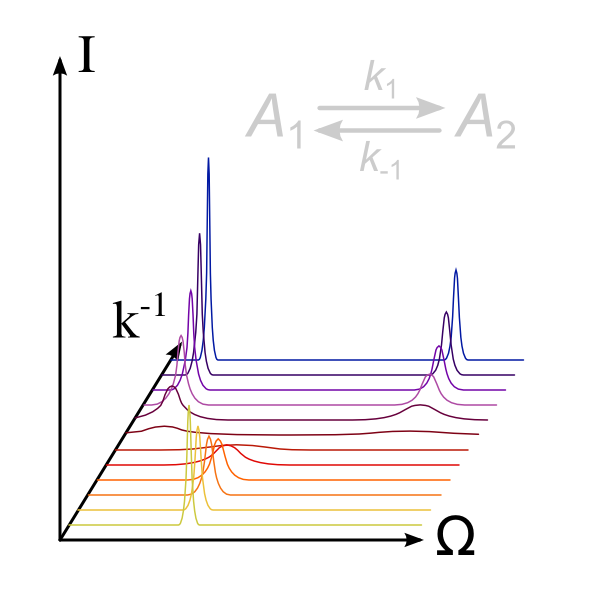
\includegraphics[width=5cm, bb=0 0 1701 1701]{graphics/analyses/relax_disp_600x600}
\end{figure*}


% Introduction.
%%%%%%%%%%%%%%%

\section{Introduction to relaxation dispersion}

Relaxation dispersion is the experimental modulation of chemical exchange relaxation.  For the $\Ronerho$-type experiment in which the nucleus of interest is spin-locked, either the spin-lock field strength or the offset between the spin-lock pulse and the chemical shift of the spins is used to modulate the exchange.  For the CPMG-type experiment, varying the time between the pulses modules the exchange.  Both experiment types are handled by relax.


% The models.
%~~~~~~~~~~~~

\subsection{The modelling of dispersion data}

The modelling of relaxation dispersion data can be catergorised into two distinct methodologies:

\begin{itemize}
\item{} Optimisation of models based on analytical, closed-form expressions derived from the Bloch-McConnell equations subject to certain conditions.
\item{} Optimisation of models via numerical integration of the Bloch-McConnell equations.
\end{itemize}

In relax currently only the optimisation of the analytic models is supported.


% Script UI.
%%%%%%%%%%%%

\section{Analysing dispersion in the prompt/script UI mode}


% The sample script.
%~~~~~~~~~~~~~~~~~~~

\subsection{Dispersion script mode -- the sample script}



% Tutorial - adding models.
%%%%%%%%%%%%%%%%%%%%%%%%%%%

\section{Tutorial for adding relaxation dispersion models}

The following is a tutorial for adding new relaxation dispersion models for either CPMG-type\index{relaxation dispersion!CPMG-type experiment} or $\Ronerho$-type\index{relaxation dispersion!$\Ronerho$-type experiment} experiments to relax.  This includes both the models based on the analytical, closed-form expressions as well as the models involving numerical integration of the Bloch-McConnell equations.  The tutorial is designed for those who feel adventurous enough to become a relax developer.  This text derives from the relax-devel@gna.org mailing list post:

\href{http://article.gmane.org/gmane.science.nmr.relax.devel/3907}{http://article.gmane.org/gmane.science.nmr.relax.devel/3907}.

The tutorial will follow the example of the addition of the `M61' model\index{relaxation dispersion!M61 model} already present within relax, pointing to the relevant commits for reference.  To see the commit message and the code changes in colour, click on the links found within these commit messages.  This specific case is the \cite{Meiboom61} analytic model for 2-site fast exchange equation for $\Ronerho$-type experiments.


\subsection{Adding the model to the list}

Reference commit:  \href{http://article.gmane.org/gmane.science.nmr.relax.scm/17611}{http://article.gmane.org/gmane.science.nmr.relax.scm/17611}

Firstly the model should be added to the lists of the \module{specific\_analyses.relax\_disp.\linebreak[0]{}variables} module.  The model name is stored in a special variable which will be used throughout relax.


\subsection{The \uf{relax\_disp.select\_model} user function front end}

Reference commit:  \href{http://article.gmane.org/gmane.science.nmr.relax.scm/17612}{http://article.gmane.org/gmane.science.nmr.relax.scm/17612}

The next step is to add the model, its description, the equations for the analytic models, and all references to the \uf{relax\_disp.select\_model} user function front end.  When the relaxation dispersion chapter of the relax manual is created (this will be the \file{docs/latex/\linebreak[0]{}relax\_disp.tex} file), then the same description should be added there as well.


\subsection{The relax library}

Reference commit:  \href{http://article.gmane.org/gmane.science.nmr.relax.scm/17615}{http://article.gmane.org/gmane.science.nmr.relax.scm/17615}

Now the dispersion function needs to be added to the relax library (in the \module{lib.relax\_disp} package).  This should be designed as a simple Python function which takes the dispersion parameters and experimental variables, and calculates the $\Rtwoeff$/$\Ronerho$ values.  The module can contain auxiliary functions for the calculation.  Some auxiliary functions, if not specific to relaxation dispersion, may be better placed in other locations within the relax library.

The relaxation dispersion functions in the library currently take as an argument a data structure for the back-calculated $\Rtwoeff$/$\Ronerho$ values and populate this structure.  This design is not essential if the target function, described in the next point, handles the library function appropriately.  Just look at the files in \module{lib.dispersion} to get an idea of the design used.

The dispersion code in the relax library must be robust.  This involves identifying parameter values or combinations which would cause failures in the mathematical operations.  Numerical issues only present in software implementation of the mathematics must be considered.  Note that parameter values of 0.0 are common within a grid search.  It should be decided whether the back-calculated $\Rtwoeff$/$\Ronerho$ value should be set to zero, to another value, or to something large (e.g. 1e$^{100}$).  For example:

\begin{description}
\item[Divisions:]  Always catch zeros in the denominator with if statements, even if you believe that this will never be encountered.
\item[Square roots:]  Make sure that the value inside is always $> 0$.
\item[Trigonometric functions:]  These should be tested for where they are not defined or where the software implementation can no longer handle certain values.  For example try math.cosh(1000) in Python.
\end{description}

In the reference example, the M61 model\index{relaxation dispersion!M61 model} code was copied from the LM63 module and modified appropriately.


\subsection{The target function}

Reference commits:

\href{http://article.gmane.org/gmane.science.nmr.relax.scm/17616}{http://article.gmane.org/gmane.science.nmr.relax.scm/17616}

\href{http://article.gmane.org/gmane.science.nmr.relax.scm/17660}{http://article.gmane.org/gmane.science.nmr.relax.scm/17660}

\href{http://article.gmane.org/gmane.science.nmr.relax.scm/17661}{http://article.gmane.org/gmane.science.nmr.relax.scm/17661}

The target function is used in optimisation and is a class method which takes as a single argument the parameter vector.  This list is changed by the minimisation algorithm during optimisation.  The target function should then return a single floating point number -- the chi-squared value.

Again in this example, the code for the M61\index{relaxation dispersion!M61 model} is copied from the LM63 model\index{relaxation dispersion!LM63 model} and then modified.


\subsection{Adding support for the parameters}

Reference commit:  \href{http://article.gmane.org/gmane.science.nmr.relax.scm/17573}{http://article.gmane.org/gmane.science.nmr.relax.scm/17573}

This is needed to enable the model.  This example is for the CR72 model\index{relaxation dispersion!CR72 model} implementation as the parameters required for the M61 model\index{relaxation dispersion!M61 model} match those of the preexisting LM63 model\index{relaxation dispersion!LM63 model}.


\subsection{The \uf{relax\_disp.select\_model} back end}

Reference commit:  \href{http://article.gmane.org/gmane.science.nmr.relax.scm/17622}{http://article.gmane.org/gmane.science.nmr.relax.scm/17622}

Now the back end of the \uf{relax\_disp.select\_model} user function for the model can be added.  This involved identifying the model and constructing the parameter list.


\subsection{The test suite}
\label{sect: test suite for dispersion}

Reference commits:

\href{http://article.gmane.org/gmane.science.nmr.relax.scm/17647}{http://article.gmane.org/gmane.science.nmr.relax.scm/17647}

\href{http://article.gmane.org/gmane.science.nmr.relax.scm/17648}{http://article.gmane.org/gmane.science.nmr.relax.scm/17648}

\href{http://article.gmane.org/gmane.science.nmr.relax.scm/17649}{http://article.gmane.org/gmane.science.nmr.relax.scm/17649}

\href{http://article.gmane.org/gmane.science.nmr.relax.scm/17662}{http://article.gmane.org/gmane.science.nmr.relax.scm/17662}

\href{http://article.gmane.org/gmane.science.nmr.relax.scm/17663}{http://article.gmane.org/gmane.science.nmr.relax.scm/17663}

This step is normally performed first.  This is the most important part that makes sure that the code not only works now, but will continue working for the entire lifetime of the relax project.

The idea is that synthetic data, here for example as Sparky\index{software!Sparky} peak lists, is created for the model and added to the test suite directory \directory{test\_suite/shared\_data/dispersion/}.  This is then used in a system test to check that the code in relax can reproduce the data.  It is very important that the code added to the relax library is not used to create the synthetic data!


\subsection{Comparing to other software}
\label{sect: dispersion software comparison}

It can happen that a bug present in the \module{lib.dispersion} package code is also replicated in the synthetic data.  This is not uncommon. Therefore it is very useful to use other software with the test data from subsection~\ref{sect: test suite for dispersion} to see if the original parameters can be found.  A good example can be seen in the test\_suite/shared\_data/dispersion/Hansen which contains Dr. Flemming Hansen's CPMG data (see the \file{README} file) and the results from different programs including NESSY\index{software!NESSY}, relax, CPMGFit\index{software!CPMGFit}, and ShereKhan\index{software!ShereKhan}.  The comparison is in the file \file{software\_comparison}.

Once the relax code is able to find identical or better results than the dispersion softwares, then the values found in the test suite optimisation can be locked in.  The assertEqual() and assertAlmostEqual() methods can be used to only allow the test to pass when the correct values are found.


\subsection{Debugging}

This step should not require an explanation.  It goes hand-in-hand with the steps of subsections~\ref{sect: test suite for dispersion} and~\ref{sect: dispersion software comparison}.
